\documentclass[11pt,a4paper]{article}
% 국문판: XeLaTeX로 컴파일한다 (latexmk -xelatex main.tex)
\usepackage[margin=1in]{geometry}
\usepackage{fontspec}
\usepackage[hangul]{kotex}
\setmainhangulfont{Noto Serif CJK KR}[ItalicFont={Noto Sans CJK KR},BoldFont={Noto Serif CJK KR Bold},BoldItalicFont={Noto Sans CJK KR Bold}]
\setsanshangulfont{Noto Sans CJK KR}
\setmonohangulfont{Noto Sans Mono CJK KR}
\usepackage{amsmath,amssymb}
\usepackage{graphicx}
\usepackage{booktabs}
\usepackage{multirow}
\usepackage{array}
\usepackage{xcolor}
\usepackage[font=small,labelfont=bf]{caption}
\usepackage{subcaption}
\usepackage[ruled,vlined,linesnumbered]{algorithm2e}
\SetAlgorithmName{알고리즘}{알고리즘}{알고리즘 목록}
\SetKwInput{KwIn}{입력}\SetKwInput{KwOut}{출력}
\usepackage{tikz}
\usetikzlibrary{arrows.meta,positioning}
\usepackage[section]{placeins}
\usepackage[numbers,sort&compress]{natbib}
\usepackage[colorlinks=true,linkcolor=blue!50!black,citecolor=blue!50!black,urlcolor=blue!50!black]{hyperref}
\usepackage[noabbrev]{cleveref}
\crefname{figure}{그림}{그림}\Crefname{figure}{그림}{그림}
\crefname{table}{표}{표}\Crefname{table}{표}{표}
\crefname{equation}{식}{식}\Crefname{equation}{식}{식}
\crefname{section}{절}{절}\Crefname{section}{절}{절}
\crefname{subsection}{절}{절}\Crefname{subsection}{절}{절}
\crefname{algocf}{알고리즘}{알고리즘}\Crefname{algocf}{알고리즘}{알고리즘}
\crefname{algorithm}{알고리즘}{알고리즘}\Crefname{algorithm}{알고리즘}{알고리즘}
\newcommand{\crefpairconjunction}{, }\newcommand{\crefmiddleconjunction}{, }\newcommand{\creflastconjunction}{, }
\newcommand{\crefpairgroupconjunction}{, }\newcommand{\crefmiddlegroupconjunction}{, }\newcommand{\creflastgroupconjunction}{, }
\crefname{appendix}{부록}{부록}
\crefformat{section}{#2#1#3절}\crefformat{subsection}{#2#1#3절}
\crefformat{figure}{그림~#2#1#3}\crefformat{table}{표~#2#1#3}\crefformat{equation}{식~(#2#1#3)}
\crefformat{algocf}{알고리즘~#2#1#3}\crefformat{algorithm}{알고리즘~#2#1#3}
\graphicspath{{../figures/}}
\newcommand{\tabdir}{../tables/ko}
\newcommand{\pct}{\,\%}
\setlength{\emergencystretch}{2em}
\linespread{1.15}

\title{\textbf{동역학 기반 결측 복원은 태양광 발전 데이터에도 통하는가?}\\[4pt]
\large 실측 PV 데이터에서의 Full-Partial Reconstruction Mapping 실증 평가}
\author{김종규\thanks{교신저자: \href{mailto:jk.kim@60hz.io}{jk.kim@60hz.io}}\\\small\href{mailto:jk.kim@60hz.io}{jk.kim@60hz.io}
\and Claude Opus 5.5\thanks{Anthropic이 개발한 AI 시스템. 논문 끝의 AI 활용 고지를 참조.}}
\date{2026년 10월}

\begin{document}
\renewcommand{\tablename}{표}\renewcommand{\figurename}{그림}\renewcommand{\abstractname}{초록}\renewcommand{\refname}{참고 문헌}
\maketitle

\begin{abstract}
태양광(PV) 모니터링 데이터의 결측은 흔하고 비용이 크지만, 실무에서는 대부분 보간이나 이웃 시스템 비율 스케일링으로 채운다.
Wu 등(Nature Communications, 2026)이 제안한 Full-Partial Reconstruction Mapping(FPRM)은 완전 관측 시계열의 지연 좌표 재구성에서 결측 시계열로 가는 사상을 가우시안 과정 회귀(GPR)로 학습해 결측을 복원한다. 원 논문은 90\pct{} 결측에서도 안정적으로 복원된다고 보고한다.
본 연구는 이 동역학 기반 접근이 태양광 데이터에도 통하는지 검증한다.
FPRM을 다시 구현하고, 원 논문의 저차원 생태계 벤치마크를 재현했다.
이어서 결측이 없는 NREL PVDAQ 데이터셋 4개(3개 현장, 1시간·15분 해상도, 시계열 4--10개)에 7가지 현실적 결측 메커니즘을 적용했다. 13개 베이스라인 및 여러 FPRM 변형과 비교했으며, 테스트셋은 본 실험 480개와 ablation 134개다.
지연 임베딩의 효과는 태양광에서도 확인된다. 같은 모델에서 임베딩만 뺀 경우보다 주간 RMSE가 중앙값 7\pct{} 낮고, 참조 시계열 31가지 모두에서 이득이 있다.
그러나 원 논문 설계(참조 1개)의 FPRM은 일반적인 결측 상황에서 테스트셋별 최강 베이스라인보다 12--16\pct{} 나쁘다. 최강 베이스라인은 주로 완전 관측 이웃 전체를 쓰는 랜덤 포레스트나 SVR이다.
완전 관측 참조를 모두 임베딩하는 확장(FPRM-multi)은 격차를 5--9\pct{}로 줄이고, 17개 기법 중 평균 순위 1위를 기록한다.
FPRM이 분명히 우세한 곳은 원 논문이 강조한 상황뿐이다. 완전 관측 시계열이 1개이고 나머지가 90\pct{} 결측이면 4개 데이터셋 모두에서 5--14\pct{} 우세하다.
반대로 고출력 구간 결측(MNAR), 시간대가 쏠린 저주기 로깅, 지역 단위 동시 장애에서는 실패한다.
결론적으로 FPRM은 태양광 데이터에서 조건부로 유용한 특화 도구이며, 본 논문은 참조 선택과 학습기 선택에 대한 구체적 지침을 제시한다.
\end{abstract}

\noindent\textbf{주제어:} 결측치 대치(imputation); 태양광 발전; 지연 임베딩; Takens 정리; 가우시안 과정 회귀; 벤치마크

\section{서론}\label{sec:intro}

운영 중인 태양광 발전소는 인버터 출력, 계량기 값, 현장 일사량으로 이뤄진 긴 다변량 시계열을 만든다.
이 시계열은 통신 장애, 로거 다운, 저주기 폴링, 센서 포화, 현장 정전 등으로 수시로 끊긴다.
결측은 발전량 정산, 성능비 추정, 열화 분석, 예측 모델 학습을 모두 왜곡하므로 결측 복원은 실무상 필수다.
실무에서는 보통 선형 보간, clear-sky index 보간, 이웃 시스템 스케일링을 쓴다.

Wu 등~\cite{wu2026fprm}은 Takens 임베딩 정리~\cite{takens1981,deyle2011}에 기반한 동역학 기반 결측 복원 틀인 \emph{Full-Partial Reconstruction Mapping}(FPRM)을 제안했다.
FPRM은 결측 시계열마다 두 개의 끌개(attractor) 재구성을 만든다.
하나는 완전 관측 시계열의 지연 좌표로 만든 \emph{완전 재구성}(full reconstruction)이고, 다른 하나는 결측 시계열 자체로 만든 \emph{부분 재구성}(partial reconstruction)이다.
두 재구성 사이의 미분동형(diffeomorphic) 사상은 가우시안 과정 회귀(GPR)로 학습한다.
원 논문은 모형계와 교통·뇌파·환율·풍속 데이터에서 최대 90\pct{} 결측 시계열을 복원했고, 통계·기계학습·동역학 기반 기존 기법보다 우수했다고 보고한다~\cite{wu2026fprm}.

태양광 출력은 이 아이디어를 적용해 볼 만하지만 쉽지 않은 대상이다.
이웃 시스템은 같은 구름장의 영향을 받으므로, 완전 관측 이웃 하나가 FPRM이 활용하는 상태 정보를 담고 있을 가능성이 높다.
반면 태양광 출력의 특성은 FPRM의 동기가 된 자율 혼돈계와 거리가 멀다.
\begin{itemize}
  \item 결정론적인 일주기 강제가 신호를 지배한다.
  \item 야간에는 정확히 0이다.
  \item 인버터 한계에서 포화된다.
  \item 값 자체와 상관된 이유로 결측되는 경우가 많다.
\end{itemize}
따라서 다음 세 질문을 던진다.
\begin{enumerate}
  \item 현실적인 태양광 결측 메커니즘에서 FPRM은 단순 실무 기법(보간, 이웃 스케일링)과 범용 기계학습 대치 기법보다 나은가?
  \item 결측률, 공백 구조, 참조 시계열 종류, 시간 해상도 중 어떤 조건에서 성공하고 어떤 조건에서 실패하는가?
  \item 실무자가 알아야 할 설정과 한계는 무엇인가?
\end{enumerate}

\paragraph{기여.}
\begin{itemize}
  \item 임베딩 파라미터를 관측값만으로 선택하는 FPRM의 공개 Python 재구현. 원 논문의 저차원 생태계 벤치마크를 재현했다(\ref{sec:synthetic}절).
  \item 결측이 없는 NREL PVDAQ 구간 4개~\cite{pvdaq}와 결측 시나리오 8종(S1--S8)으로 구성한 태양광 결측 복원 벤치마크(\ref{sec:setup}절). 무작위, 블록, 하루 단위, 주기, 임계값(MNAR), 단일 참조, 동시 결측, 참조 선택을 다룬다.
  \item 테스트셋 614개에서 FPRM, 그 변형, 베이스라인 13종을 대응 표본 유의성 검정과 함께 비교했다(\ref{sec:results}절).
  \item 지연 임베딩은 태양광 데이터에서도 이득이지만, 원 논문의 단일 참조 설계는 일반 회귀기가 활용하는 정보를 버린다는 근거. 전체 참조 확장(FPRM-multi)이 격차 대부분을 메운다.
  \item 실무 지침(\ref{sec:discussion}절):
  \begin{itemize}
    \item 참조로는 일사계보다 상관이 가장 높은 이웃 \emph{출력} 시계열을 쓴다.
    \item 학습기로는 GPR 대신 SVR을 쓴다(정확도 동일, 약 45배 빠름).
    \item 결측 패턴에 따라 복원 방법을 분기한다.
  \end{itemize}
\end{itemize}

\section{관련 연구}\label{sec:related}

\paragraph{결측 이론과 범용 대치 기법.}
결측 메커니즘은 완전 무작위 결측(MCAR), 무작위 결측(MAR), 비무작위 결측(MNAR)으로 나뉜다~\cite{rubin1976,little2019}.
널리 쓰이는 범용 대치 기법으로 연쇄 방정식 다중대치(MICE)~\cite{vanbuuren2011}, $k$-최근접 이웃 대치~\cite{troyanskaya2001}, 랜덤 포레스트 기반 대치~\cite{breiman2001,stekhoven2012}가 있다.
GAIN~\cite{yoon2018gain}, BRITS~\cite{cao2018brits}, SAITS~\cite{du2023saits} 같은 딥러닝 생성·순환 모델 기반 기법은 대규모 학습 데이터에서 시간 구조와 시계열 간 구조를 학습한다.
본 연구는 MICE와 $k$NN 대치를 다변량 베이스라인으로 포함하고, 딥러닝 기법은 후속 과제로 남긴다(\ref{sec:limitations}절).

\paragraph{상태공간 재구성.}
Takens 정리~\cite{takens1981}와 그 다변량 일반화~\cite{deyle2011}는 단일 관측량의 지연 좌표로 원 끌개와 미분동형인 끌개를 재구성할 수 있음을 보장한다.
임베딩 파라미터는 고전적으로 자기 상호정보량(AMI)의 첫 극소~\cite{fraser1986}와 거짓 최근접 이웃(FNN) 기준~\cite{kennel1992}으로 고른다.
경험적 동역학 모델링은 이를 토대로 발전했다.
\begin{itemize}
  \item S-map~\cite{sugihara1994}: 재구성 공간에서 국소 가중 선형 예측을 한다.
  \item 수렴 교차사상(CCM)~\cite{sugihara2012}: 재구성을 인과 추론에 활용한다.
  \item 다중 관점 임베딩(MVCM)~\cite{ye2016}: 여러 임베딩을 결합한다.
\end{itemize}
FPRM~\cite{wu2026fprm}은 이런 이웃 기반 방법과 달리 완전·부분 재구성 사이의 전역 사상을 GPR~\cite{rasmussen2006}로 학습한다.

\paragraph{태양광 데이터.}
pvlib~\cite{holmgren2018pvlib}에 구현된 Ineichen--Perez 모형~\cite{ineichen2002} 같은 clear-sky 모형은 태양광 출력과 일사량 정규화의 표준 도구다.
clear-sky index와 이웃 비율 스케일링은 사실상의 실무 결측 보정 기준선이며, 본 연구도 둘 다 포함한다.
우리가 아는 범위에서, 통제된 현실적 결측 조건으로 태양광 데이터에서 동역학 기반 대치를 평가한 연구는 없다.

\section{방법}\label{sec:method}

\subsection{Full-Partial Reconstruction Mapping}

$x_i(t)$, $t=1,\dots,l$을 완전 관측 시계열, $x_j(t)$를 결측 시계열이라 하자.
임베딩 차원 $E$와 지연 $\tau$에 대해 완전 재구성은 다음과 같다.
\begin{equation}
  \mathbf{X}_i(t) = \big(x_i(t),\,x_i(t+\tau),\,\dots,\,x_i(t+(E-1)\tau)\big),\qquad t = 1,\dots,m,\; m = l-(E-1)\tau .
  \label{eq:full}
\end{equation}
부분 재구성 $\mathbf{X}_j(t)$도 $x_j$로 같은 방식으로 정의하며, 일부 좌표가 결측이다.
Takens 정리에 따르면 두 재구성 모두 계의 끌개 $M$과 미분동형이다($f:M\to M(x_i)$, $g:M\to M(x_j)$).
따라서 매끄러운 사상 $F = g\circ f^{-1}: M(x_i)\to M(x_j)$가 존재한다.
FPRM은 이 사상의 첫 좌표
\begin{equation}
  x_j(t) = F\big(\mathbf{X}_i(t)\big)
  \label{eq:map}
\end{equation}
를 $x_j(t)$가 관측된 시점들에서 학습하고, 결측 시점 $k$에서 $\hat x_j(k) = F(\mathbf{X}_i(k))$로 복원한다~\cite[식 11--14]{wu2026fprm}.

$F$는 가우시안 과정이다.
커널은 제곱지수 커널 $q(\mathbf{x},\mathbf{x}') = \exp\!\big(-\lVert\mathbf{x}-\mathbf{x}'\rVert^2/2\theta^2\big)$이고, 척도 $\theta$는 예측변수 표준편차의 평균으로 초기화한다. 여기에 가우시안 잡음 $\sigma^2$을 더한다.
사후 평균은
\begin{equation}
  u_*(\tilde{\mathbf{x}}) = u(\tilde{\mathbf{x}}) + q(\tilde{\mathbf{x}},\mathbf{X})\,\big(q(\mathbf{X},\mathbf{X})+\sigma^2 I\big)^{-1}\big(\mathbf{y}-u(\mathbf{X})\big)
  \label{eq:gp}
\end{equation}
이며, $u$는 상수 평균 함수다~\cite[식 15--18]{wu2026fprm}.
결측 시계열마다 별도의 사상을 학습한다. \Cref{fig:pipeline}에 전체 절차를 요약했다.

\begin{figure}[t]
  \centering
  \newcommand{\PLa}{\textbf{완전 시계열} $x_i$}
  \newcommand{\PLb}{\textbf{결측 시계열} $x_j$}
  \newcommand{\PLc}{\textbf{완전 재구성}}
  \newcommand{\PLd}{\textbf{학습 쌍}}
  \newcommand{\PLe}{\textbf{사상 $F$ 학습}}
  \newcommand{\PLf}{\textbf{복원}}
  \newcommand{\PLg}{지연 임베딩}
  \newcommand{\PLh}{결측 시점 $k$}
  \resizebox{\linewidth}{!}{% FPRM pipeline schematic (shared by en/ko; labels passed via macros \PLa ... \PLh)
\begin{tikzpicture}[
  font=\footnotesize, >=Stealth,
  box/.style={draw=black!60, rounded corners=2pt, fill=#1, align=center, minimum height=1.05cm, inner sep=3pt},
  box/.default=white]
  \definecolor{cblue}{HTML}{2a78d6}\definecolor{corange}{HTML}{eb6834}\definecolor{cgray}{HTML}{f0efec}
  % reference series
  \node[box=cblue!8, text width=2.6cm] (ref) at (0,0) {\PLa\\[2pt]
    \begin{tikzpicture}[x=0.22cm,y=0.22cm]\draw[cblue,thick] plot[smooth] coordinates {(0,0)(1,1.4)(2,2.1)(3,1.5)(4,0.3)(5,0)(6,1.2)(7,2.2)(8,1.6)(9,0.2)};\end{tikzpicture}};
  % incomplete series
  \node[box=corange!8, text width=2.6cm] (tgt) at (0,-2.3) {\PLb\\[2pt]
    \begin{tikzpicture}[x=0.22cm,y=0.22cm]\draw[corange,thick] plot[smooth] coordinates {(0,0)(1,1.2)(2,1.9)}; \draw[corange,thick,dashed,opacity=.45] plot[smooth] coordinates {(2,1.9)(3,1.4)(4,0.3)(5,0)(6,1.0)}; \draw[corange,thick] plot[smooth] coordinates {(6,1.0)(7,2.0)(8,1.4)(9,0.2)};\end{tikzpicture}};
  % full reconstruction
  \node[box, text width=3.6cm] (full) at (5.1,0) {\PLc\\[1pt] $\mathbf{X}_i(t)=\big(x_i(t),\,x_i(t{+}\tau),$\\ $\dots,\,x_i(t{+}(E{-}1)\tau)\big)$};
  % training pairs
  \node[box=cgray, text width=3.6cm] (pairs) at (5.1,-2.3) {\PLd\\[1pt] $\{(\mathbf{X}_i(t),x_j(t)) : x_j(t)\ \text{observed}\}$};
  % mapping
  \node[box=cblue!8, text width=2.9cm] (map) at (9.4,-1.15) {\PLe\\[1pt] $x_j(t)=F(\mathbf{X}_i(t))$\\ GPR / SVR / MLP};
  % output
  \node[box=corange!8, text width=2.5cm] (out) at (14.1,-1.15) {\PLf\\[1pt] $\hat x_j(k)=F(\mathbf{X}_i(k))$};
  \draw[->,thick,black!60] (ref) -- node[above,font=\scriptsize]{\PLg} (full);
  \draw[->,thick,black!60] (full) -- (pairs);
  \draw[->,thick,black!60] (tgt) -- (pairs);
  \draw[->,thick,black!60] (pairs.east) -- (map.south west);
  \draw[->,thick,black!60] (full.east) -- (map.north west);
  \draw[->,thick,black!60] (map) -- node[above,font=\scriptsize]{\PLh} (out);
\end{tikzpicture}
}
  \caption{FPRM 절차. 완전 관측 참조 시계열을 지연 임베딩한다(\cref{eq:full}). 지연 벡터와 같은 시각에 관측된 결측 시계열 값의 쌍으로 회귀 사상 $F$를 학습하고(\cref{eq:map}), 결측 시점의 지연 벡터에서 $F$를 평가한다. 원 논문은 $F$로 GPR을 쓰며, 본 연구는 SVR과 MLP도 시험한다.}
  \label{fig:pipeline}
\end{figure}

\subsection{구현}\label{sec:impl}

원 구현은 figshare에 공개된 MATLAB 코드다~\cite{wu2026fprm}.
우리 실행 환경에서는 접근할 수 없었으므로, 원 논문의 서술을 바탕으로 scikit-learn~\cite{pedregosa2011}을 사용해 Python으로 다시 구현했다(\cref{alg:fprm}).
원 논문이 정하지 않은 설계 결정은 다음과 같다.

\begin{itemize}
  \item \textbf{GPR.}
  \begin{itemize}
    \item 커널은 상수 $\times$ RBF $+$ 백색잡음이고 \texttt{normalize\_y}를 쓴다. MATLAB \texttt{fitrgp}의 기본값(제곱지수 커널, 상수 기저, 초기 척도 = 예측변수 표준편차 평균)을 따른 것이다.
    \item 하이퍼파라미터는 \emph{중복을 제거한} 학습 행 최대 600개에서 주변 우도를 최대화해 정한다(재시작 1회, 상대 잡음 하한 $10^{-4}$).
    \item 최종 정확 GP는 학습점을 최대 2{,}000개까지 쓴다(subset of data, \texttt{fitrgp}의 $n>2000$일 때 동작과 같음).
  \end{itemize}
  \item \textbf{야간 행.} 태양광 데이터에는 똑같은 야간 행이 수천 개 있다. 중복을 제거하지 않으면 우도가 잡음 0, 극소 길이척도의 보간해로 수렴했다. 그 결과 직접 GPR이 무너졌다(한 테스트셋에서 상관 0.99 대신 0.70). GP 기반 태양광 대치에서 실무적으로 주의할 함정이다.
  \item \textbf{임베딩 파라미터.} 원 논문의 선택 방법(보충자료 Fig.~S1)은 구할 수 없었다. 대신 \emph{관측된} 목표값의 무작위 1/3을 검증용으로 두고 격자 탐색으로 $(E,\tau)$를 고른다($E\in\{1,2,3,4,6,8\}$, $\tau\in\{1,2,4\}$ step). 정답 값은 전혀 쓰지 않는다. AMI/FNN 선택기~\cite{fraser1986,kennel1992}도 구현했다.
  \item \textbf{참조 선택.} 원 논문은 완전 시계열이 하나 있다고 가정한다. 본 구현의 기본 FPRM은 관측 구간에서 목표와 상관이 가장 높은 완전 시계열을 참조로 쓴다.
  \item \textbf{예측 불가 행.} 참조 자체가 결측이면(S7) 지연 벡터를 만들 수 없다. 이런 행은 clear-sky index 보간으로 채우고 개수를 기록한다. 원 논문의 lag-FPRM 확장(보충자료 Fig.~S15--S17)은 구할 수 없어 구현하지 않았다.
\end{itemize}

원 논문에 \emph{없는} 변형 세 가지도 함께 평가한다. 표에서는 $\dagger$로 표시한다.
\begin{itemize}
  \item FPRM-multi$^\dagger$: 모든 완전 시계열의 지연 벡터를 이어 붙인다.
  \item FPRM-back$^\dagger$: 실시간으로 쓸 수 있는 인과적 임베딩 $(x_i(t), x_i(t-\tau),\dots)$이다.
  \item FPRM-csi$^\dagger$: clear-sky index $k = P/(s\cdot\mathrm{GHI}_{cs})$ 공간에서 FPRM을 적용하고 역변환한다.
\end{itemize}

\begin{algorithm}[t]
\caption{결측 시계열 하나에 대한 FPRM 복원(본 구현)}\label{alg:fprm}
\KwIn{결측을 NaN으로 표시한 데이터 행렬 $X\in\mathbb{R}^{T\times n}$; 목표 열 $j$; 완전 관측 열 집합 $\mathcal{C}$}
\KwOut{복원된 열 $\hat x_j$}
$Z \leftarrow$ 관측값 통계만으로 $X$를 z-점수화\;
$\mathcal{R} \leftarrow \arg\max_{i\in\mathcal{C}\setminus\{j\}} |\mathrm{corr}(z_i,z_j)|$ \tcp*{FPRM-multi: $\mathcal{R}\leftarrow\mathcal{C}\setminus\{j\}$}
\ForEach{격자의 $(E,\tau)$}{
  \cref{eq:full}로 $\mathbf{X}_{\mathcal{R}}(t)$ 구성; 관측 $t$의 2/3로 $F$ 학습; 나머지 1/3에서 RMSE 평가\;
}
$(E^*,\tau^*) \leftarrow$ 최적 점수\;
$\mathcal{O}\leftarrow\{t: z_j(t)\ \text{관측}\}$, $\mathcal{M}\leftarrow\{t: z_j(t)\ \text{결측},\ \mathbf{X}_{\mathcal{R}}(t)\ \text{유한}\}$\;
$\{(\mathbf{X}_{\mathcal{R}}(t), z_j(t))\}_{t\in\mathcal{O}}$로 $F$ 학습(GPR, \cref{eq:gp})\;
$k\in\mathcal{M}$에 대해 $\hat z_j(k) \leftarrow F(\mathbf{X}_{\mathcal{R}}(k))$; 남은 결측 $\leftarrow$ 대체 방법\;
\Return 표준화를 되돌린 $\hat z_j$\;
\end{algorithm}

\section{실험 설정}\label{sec:setup}

\subsection{데이터}

모든 데이터는 NREL PVDAQ~\cite{pvdaq}의 실측 AC 출력이며, 공개 OEDI S3 버킷에서 받았다.
다른 후보 소스(NREL 웹 서비스, DKASC, PVGIS, 한국 공공데이터포털)는 실행 환경의 네트워크 정책으로 차단되었다.
남긴 모든 시계열이 완전 관측인 구간 4개를 구성해, 원래 값을 정답으로 쓸 수 있게 했다(\cref{tab:datasets}).
\begin{itemize}
  \item 플로리다주 St.\ Petersburg의 상업 건물 지붕 4곳(공간 군집).
  \item 루이지애나주 New Orleans의 주택 지붕 10곳. 방위가 제각각이라 일중 최대 출력 시각이 현지 시각 10--13시에 걸쳐 있다.
  \item Maui의 한 현장. 수평면 전일사량(GHI) 일사계 1개와 스트링 인버터 7--8개로 구성되며, 1시간과 15분 해상도 두 가지로 만들었다.
\end{itemize}
상관은 다음과 같다.
\begin{itemize}
  \item St.\ Petersburg: 쌍별 상관 0.98--0.99.
  \item New Orleans: 쌍별 상관의 중앙값 0.92 이상.
  \item Maui 인버터 간: 0.97--0.99.
  \item Maui GHI 일사계와 인버터 간: 0.90--0.94에 그친다.
\end{itemize}

전처리는 다음과 같다.
\begin{itemize}
  \item 모든 시각을 UTC로 바꿨다. Maui의 인버터와 일사계 시계는 pvlib clear-sky GHI~\cite{holmgren2018pvlib,ineichen2002}와의 상관이 최대가 되도록 각각 맞췄다.
  \item 인버터는 야간에 기록하지 않으므로, 야간 공백(태양 천정각 $\ge 90^\circ$)은 0으로 채웠다.
  \item 2 step 이하 공백만 메웠고, 그보다 긴 공백이 있는 열은 제외했다.
  \item 죽었거나 고장 났거나 시계가 어긋난 채널은 점검 후 제외했다: Maui \texttt{inv05}/\texttt{inv06}, St.\ Petersburg 1321/1329, New Orleans 1268/1273.
  \item 각 시계열의 명목 용량은 관측값의 99.9 백분위수로 정했다.
\end{itemize}

\begin{table}[t]
  \centering\small
  \caption{데이터셋. 모든 구간은 야간 보정 후 결측이 없다. ``참조''는 S6과 FPRM-ref에서 쓰는 지정 참조다.}
  \label{tab:datasets}
  \resizebox{\linewidth}{!}{\input{\tabdir/datasets}}
\end{table}

\subsection{결측 시나리오}

시나리오는 \cref{tab:scenarios}에 정리했다.
\begin{itemize}
  \item S1--S5: 비참조 시계열의 절반(무작위)을 결측 시계열로 만들고 나머지는 완전 관측으로 둔다.
  \item S6: 지정 참조만 완전 관측으로 남긴다. Wu 등이 강조한 상황이다.
  \item S7: 참조를 포함한 모든 시계열에서 같은 블록을 지운다.
  \item S8: 각 시계열을 차례로 유일한 완전 참조로 삼는다.
\end{itemize}
모든 마스크는 (데이터셋, 시나리오, 파라미터, seed)로 결정되며, 설정마다 seed 5개를 쓴다.
본 실험은 데이터셋 4개 $\times$ 파라미터 설정 24개 $\times$ seed 5개 $=$ 테스트셋 480개다.
ablation은 설정 6개 $\times$ seed 3개(72개), S8 스윕은 참조 31개 $\times$ seed 2개(62개)다.
S1의 $r=0.9$에서 평균 공백 길이는 2.5--10시간, 최장 공백은 86시간에 이른다.

\begin{table}[t]
  \centering\small
  \caption{결측 시나리오. MCAR: 완전 무작위 결측, MNAR: 비무작위 결측.}
  \label{tab:scenarios}
  \resizebox{\linewidth}{!}{\input{\tabdir/scenarios}}
\end{table}

\subsection{베이스라인, 지표, 통계}

비교 기법은 \cref{tab:methods}와 같다.
직접 ML 회귀기는 모든 완전 시계열의 \emph{현재} 값을 입력으로 받는다. 따라서 단일 참조 FPRM보다 더 많은 시계열을 쓰지만 지연 좌표는 쓰지 않는다.

모든 기법에 같은 후처리를 적용한다. 음수는 0으로 자르고, 태양 천정각이 $90^\circ$ 이상이면 출력을 0으로 둔다.
야간의 0값은 모든 점수를 부풀리므로, 지표는 제거된 값 중 \emph{주간}(천정각 $<85^\circ$) 시점에서만 계산한다.

주 지표는 명목 용량 대비 RMSE(\%cap)다.
원 논문의 지표~\cite[식 19]{wu2026fprm}인 Pearson $\rho$와 정답 표준편차로 정규화한 RMSE도 보고한다.
그 밖에 MAE, 편향(bias), 결측 구간 총에너지의 절대 오차를 계산한다.

모델 선택과 $(E,\tau)$ 선택은 제거된 값을 보지 않는다. 숨긴 값을 바꿔도 출력이 변하지 않음을 단위 테스트로 확인했다.
유의성은 (seed $\times$ 시계열) 쌍에 대한 대응 Wilcoxon 부호 순위 검정~\cite{wilcoxon1945}으로 판단한다.
St.\ Petersburg는 S1--S5에서 결측 시계열이 1개라 쌍이 5개뿐이고, 검정력이 낮다.

\begin{table}[t]
  \centering\small
  \caption{비교 기법. $^\dagger$: 원 논문에 없는 확장.}
  \label{tab:methods}
  \input{\tabdir/methods}
\end{table}

\section{결과}\label{sec:results}

\subsection{모형계 재현}\label{sec:synthetic}

먼저 원 논문의 3차원 생태계와 Lorenz 계~\cite{lorenz1963}에서 구현을 점검했다(\cref{tab:synthetic,fig:synthetic}).
두 계 모두 $x$는 완전 관측이고, $y$와 $z$는 값의 비율 $r$을 무작위로 잃는다(20회 반복).
\begin{itemize}
  \item 생태계에서는 본 구현의 FPRM이 원 논문과 일치한다($r=0.9$에서 $\rho\approx0.99$).
  \item Lorenz 계에서는 보고된 값보다 훨씬 좋았고, 표본 간격을 3배로 늘려도 마찬가지였다.
  \item 원 논문이 Lorenz의 표본 간격, 잡음, $(E,\tau)$를 충분히 밝히지 않아 차이의 원인은 특정할 수 없다.
  \item 흥미롭게도 임베딩 \emph{없는} GPR이 원 논문의 Lorenz $y$ 수치를 재현한다(0.89/0.46 대 0.90/0.48).
  \item 모든 경우 임베딩을 빼면 성능이 무너진다($\rho=0.18$--0.65). 성능을 만드는 것이 회귀기가 아니라 메커니즘임을 확인해 준다.
\end{itemize}

\begin{table}[t]
  \centering\small
  \caption{$r=0.9$에서의 모형계 재현: 20회 반복 평균 Pearson $\rho$ / 정규화 RMSE. 논문 값은 Wu 등~\cite{wu2026fprm}(Fig.~3 및 본문)에서 인용.}
  \label{tab:synthetic}
  \input{\tabdir/synthetic}
\end{table}

\begin{figure}[t]
  \centering
  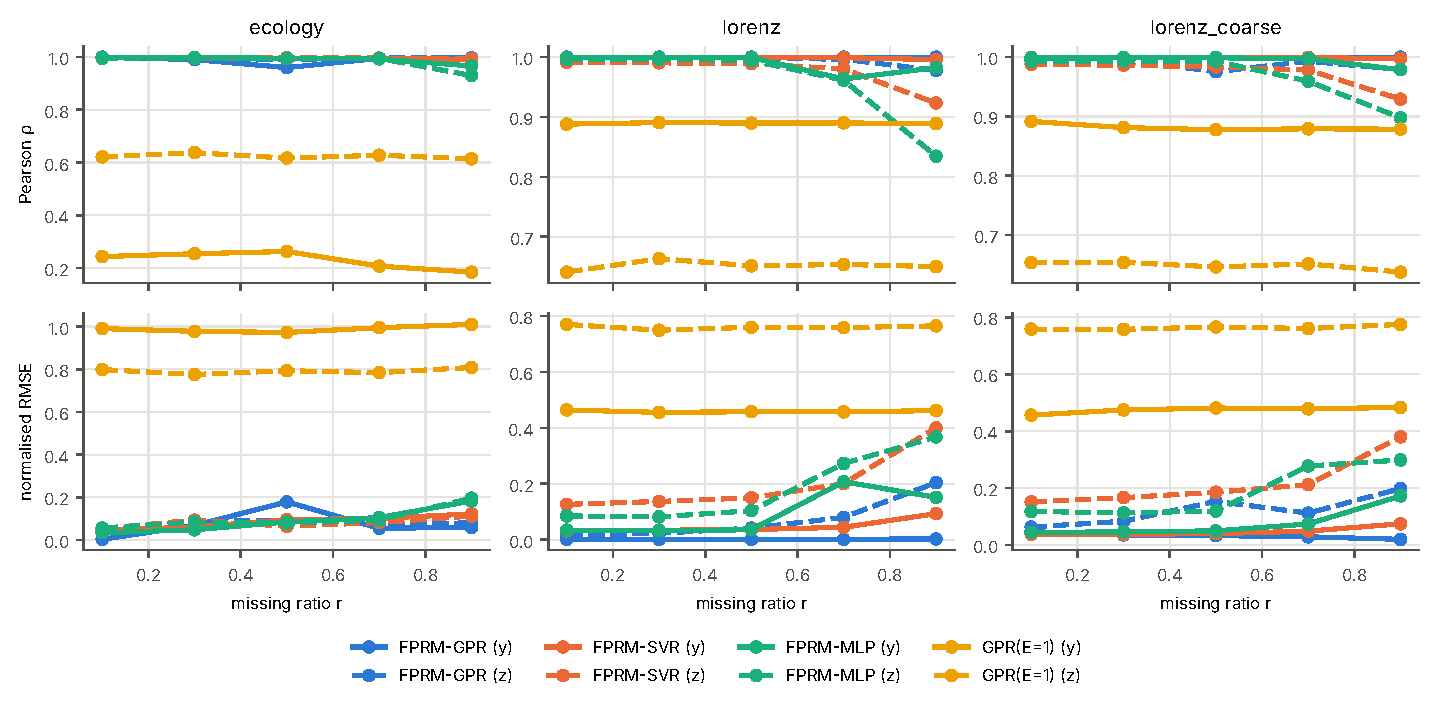
\includegraphics[width=\linewidth]{synthetic_reproduction.pdf}
  \caption{결측률 $r$에 따른 모형계 재현 결과(실선: $y$, 점선: $z$; 20회 반복). 위: Pearson $\rho$, 아래: 정규화 RMSE. GPR·SVR·MLP 사상을 쓴 FPRM은 $\rho=1$ 부근을 유지하지만, $x$의 현재 값만 쓰는 GPR($E=1$)은 실패한다.}
  \label{fig:synthetic}
\end{figure}

\subsection{태양광 데이터 전체 비교}

\Cref{tab:rank}는 17개 기법을 (테스트셋, 시계열) 쌍마다 RMSE로 순위 매긴 결과다.
\Cref{tab:median}은 RMSE 중앙값이고, \cref{fig:curves}는 결측률과 공백 길이에 따른 RMSE 변화다.
네 가지가 두드러진다.
\begin{enumerate}
  \item 일반 시나리오(S1--S3)에서는 회귀 계열 기법 모두 $\rho\approx0.98$이다. 이들 사이의 RMSE 차이(약 1\pct{}cap)는 상관 기반 평가로는 보이지 않는다.
  \item 같은 시나리오에서는 모든 완전 이웃을 쓰는 RF, SVR, MLP가 가장 강하다(평균 순위 3.6--5.3).
  \item 단일 참조 FPRM은 6.9--7.4위다. 그래도 임베딩을 뺀 FPRM-E1(9.6--10.0위)보다는 일관되게 낫다.
  \item 전체 평균 순위 1위는 FPRM-multi다(5.7).
\end{enumerate}
이웃이 있으면 보간 계열 기법(Linear, CSI-Linear, Diurnal)은 크게 뒤처지고, 공백이 길어질수록 오차가 빠르게 커진다(\cref{fig:curves}b).
S1--S3에서 결측 구간 에너지 오차는 FPRM과 ML 회귀기 모두 1\pct{} 미만이다(부록 \cref{tab:energy}).

\begin{table}[t]
  \centering\small
  \caption{시나리오별 평균 순위(17개 중 1 = 최고). (테스트셋, 결측 시계열)마다 RMSE(\%cap)로 매겼다. 굵은 글씨: 열별 최고.}
  \label{tab:rank}
  \input{\tabdir/rank}
\end{table}

\begin{table}[t]
  \centering\small
  \caption{주간 RMSE(용량 대비 \%)의 중앙값. 모든 데이터셋, seed, 시계열을 통틀어 계산했다. S7에서는 참조가 없어 대부분 기법이 CSI-Linear 대체 결과(24.2)와 같다. 굵은 글씨: 열별 최고.}
  \label{tab:median}
  \input{\tabdir/median_rmse}
\end{table}

\begin{figure}[t]
  \centering
  \begin{subfigure}{\linewidth}\centering
    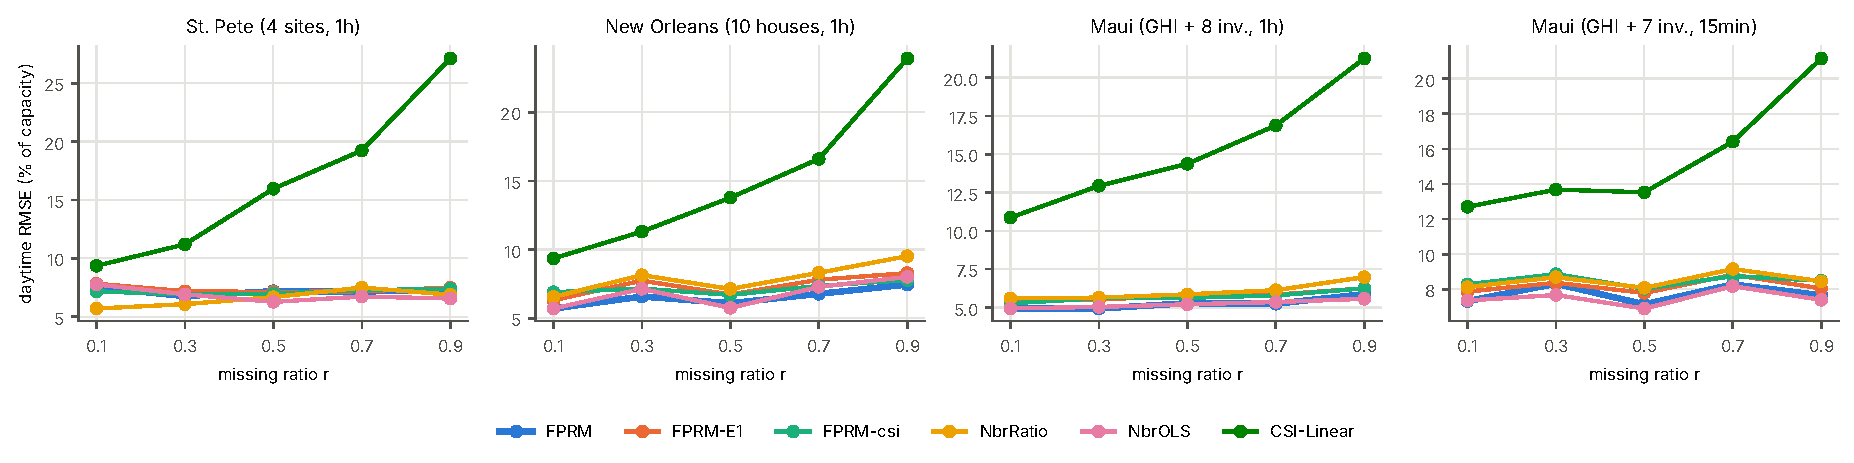
\includegraphics[width=\linewidth]{s1_mcar_curves.pdf}\caption{S1: 무작위 결측, 결측률 $r$.}
  \end{subfigure}\\[4pt]
  \begin{subfigure}{\linewidth}\centering
    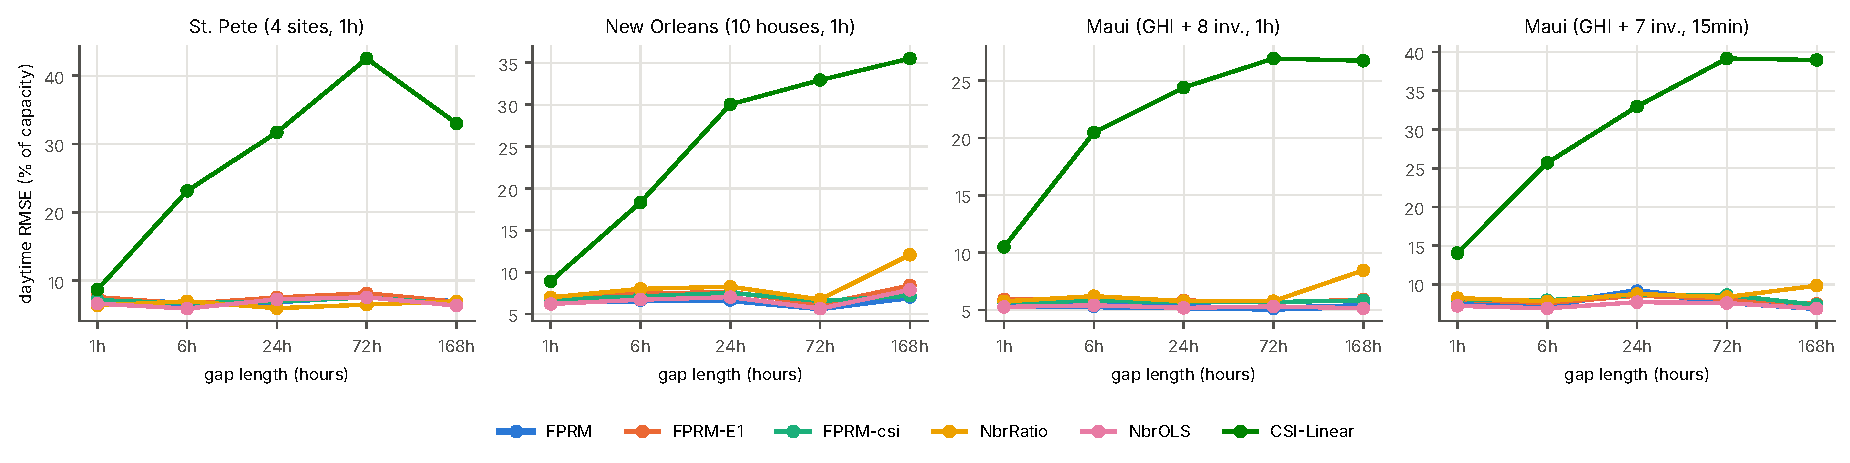
\includegraphics[width=\linewidth]{s2_block_curves.pdf}\caption{S2: 길이 $L$의 연속 공백(결측 20\pct{}).}
  \end{subfigure}
  \caption{4개 데이터셋에서 FPRM, 그 변형, 실무 베이스라인의 주간 RMSE(\%cap; seed와 결측 시계열 평균). FPRM은 FPRM-E1보다 일관되게 낮아 임베딩의 이득을 보여 주며, 이웃 회귀(NbrOLS)와는 대체로 비슷하다. clear-sky index 보간은 공백이 길어지면 빠르게 나빠진다.}
  \label{fig:curves}
\end{figure}

\subsection{최강 베이스라인과의 비교}

(데이터셋, 시나리오, 파라미터) 셀마다 FPRM을 그 셀에서 가장 좋았던 비-FPRM 기법(13개 중)과 비교했다(\cref{tab:family,fig:heatmap}).
셀별 사후(oracle) 선택은 의도적으로 FPRM에 불리한 비교이며, 고정된 기법끼리의 비교는 평균 순위(\cref{tab:rank})가 보여 준다.

S1--S3 결과는 다음과 같다.
\begin{itemize}
  \item 단일 참조 FPRM은 중앙값 기준 12--16\pct{} 나쁘다. 52개 셀 중 1개에서 이기고 35개에서 유의하게 진다.
  \item FPRM-multi는 중앙값 기준 5--9\pct{} 나쁘다. 18개 셀에서 이기고(유의 7), 15개에서 유의하게 진다.
\end{itemize}
S4와 S7을 제외한 모든 시나리오에서 FPRM은 FPRM-E1보다 중앙값 0.5--7.6\pct{} 낫다.

\begin{table}[t]
  \centering\small
  \caption{FPRM과 FPRM-multi를 (데이터셋, 시나리오, 파라미터) 셀별 최강 비-FPRM 베이스라인과 비교. ``중앙 상대오차''는 RMSE 상대 차이의 중앙값이며 음수면 FPRM이 우세하다. 유의성: 대응 Wilcoxon $p<0.05$.}
  \label{tab:family}
  \resizebox{\linewidth}{!}{\input{\tabdir/family}}
\end{table}

\begin{figure}[t]
  \centering
  \begin{subfigure}{0.49\linewidth}\centering
    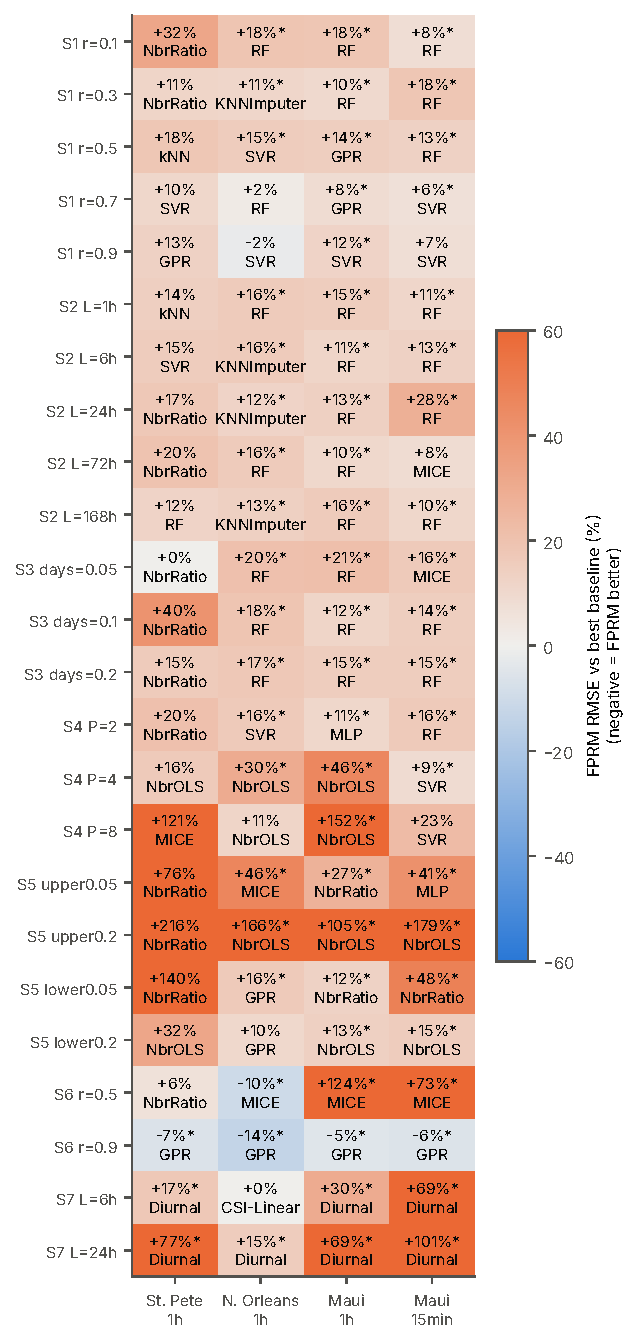
\includegraphics[width=\linewidth]{fprm_vs_best_heatmap.pdf}\caption{FPRM(원 논문 설계)}
  \end{subfigure}\hfill
  \begin{subfigure}{0.49\linewidth}\centering
    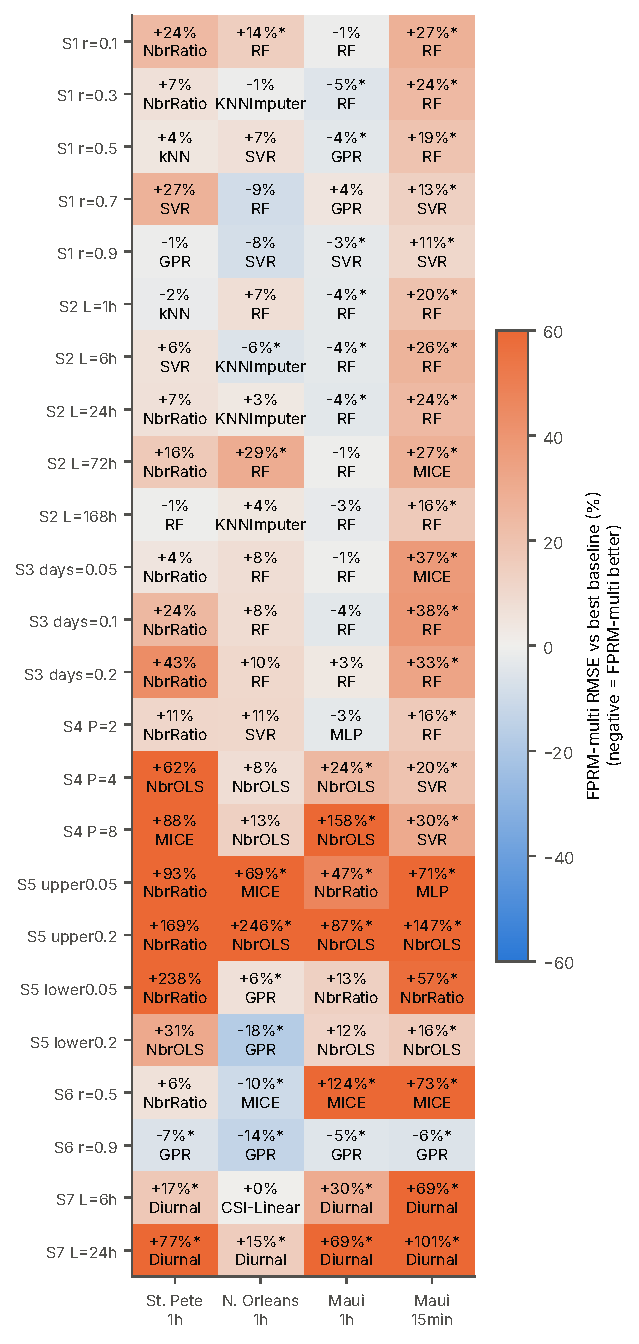
\includegraphics[width=\linewidth]{fprm_multi_vs_best_heatmap.pdf}\caption{FPRM-multi$^\dagger$}
  \end{subfigure}
  \caption{각 테스트 셀의 최강 비-FPRM 기법 대비 FPRM의 상대 RMSE. 파랑은 FPRM 우세, 주황은 열세이고, $^*$는 대응 Wilcoxon $p<0.05$, 칸 안의 이름은 최강 베이스라인이다. FPRM은 S6 $r=0.9$와 New Orleans 일부 셀에서만 이긴다. 열세는 S4(주기), S5(임계값), S7(동시 결측)에 몰려 있다.}
  \label{fig:heatmap}
\end{figure}

\subsection{완전 관측 시계열이 하나뿐일 때(S6)}

S6은 Wu 등이 FPRM의 우위가 가장 크다고 보고한 상황이다.
$r=0.9$에서 FPRM은 4개 데이터셋 모두에서 최고다. 최강 베이스라인보다 5--14\pct{} 낫고, 모든 경우 유의하다(\cref{tab:s6,fig:s6}).
정보가 희소할 때는 단일 참조의 지연 좌표가 가장 정보가 많은 입력이다.

$r=0.5$에서는 양상이 달라진다.
\begin{itemize}
  \item Maui에서는 MICE가 큰 차이로 이긴다(7.0 대 15.7\pct{}cap).
  \item MICE는 시각마다 \emph{부분적으로} 관측된 이웃까지 활용하지만, FPRM은 완전 시계열만 입력으로 받아 이들을 버린다.
  \item 게다가 Maui에서는 유일한 완전 시계열이 GHI 일사계라서 MICE를 뺀 모든 기법이 불리하다(\ref{sec:ablation}절).
\end{itemize}
\Cref{fig:example}은 맑은 날, 흐린 날, 변동이 큰 날의 S6 복원 예다.

\begin{table}[t]
  \centering\small
  \caption{S6(지정 참조만 완전 관측): RMSE(\%cap), seed 5개와 모든 결측 시계열의 평균. 굵은 글씨: 나열한 기법 중 행별 최고. 마지막 열은 베이스라인 13개 전체 중 최고.}
  \label{tab:s6}
  \resizebox{\linewidth}{!}{\input{\tabdir/s6}}
\end{table}

\begin{figure}[t]
  \centering
  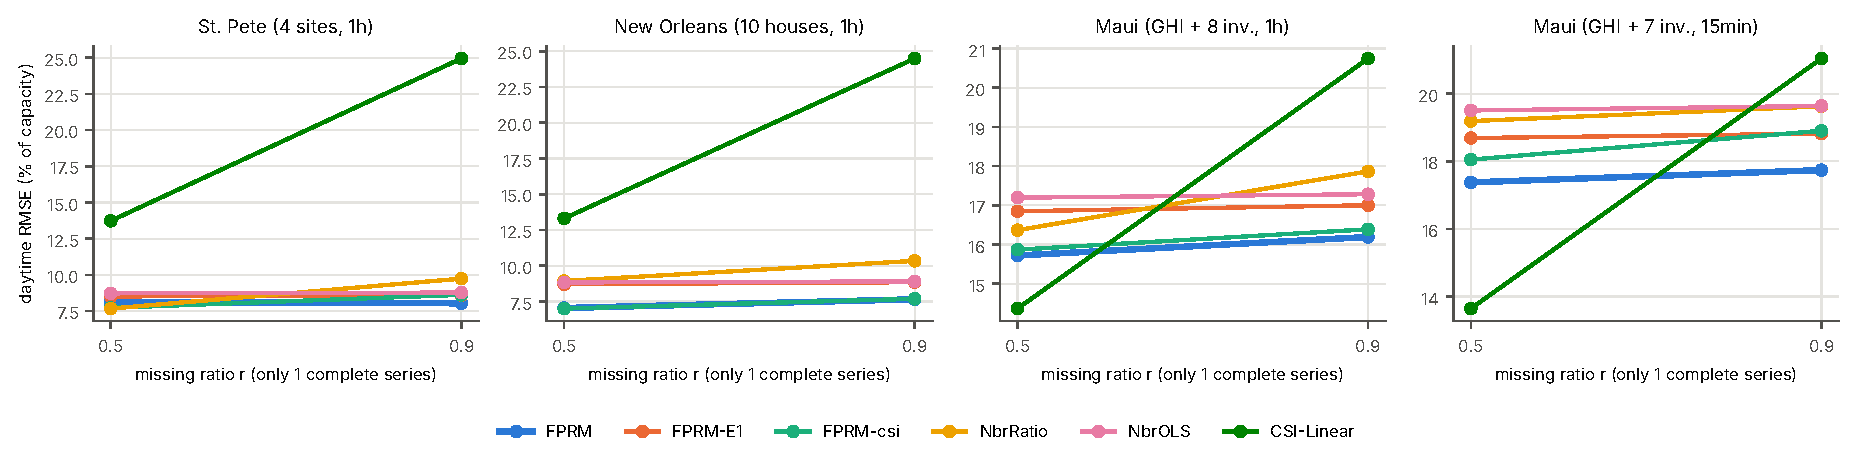
\includegraphics[width=\linewidth]{s6_oneref_curves.pdf}
  \caption{S6: 완전 시계열 1개, 나머지 결측률 50\pct{}와 90\pct{}에서의 주간 RMSE. $r=0.9$에서는 모든 데이터셋에서 FPRM이 가장 낮다.}
  \label{fig:s6}
\end{figure}

\begin{figure}[t]
  \centering
  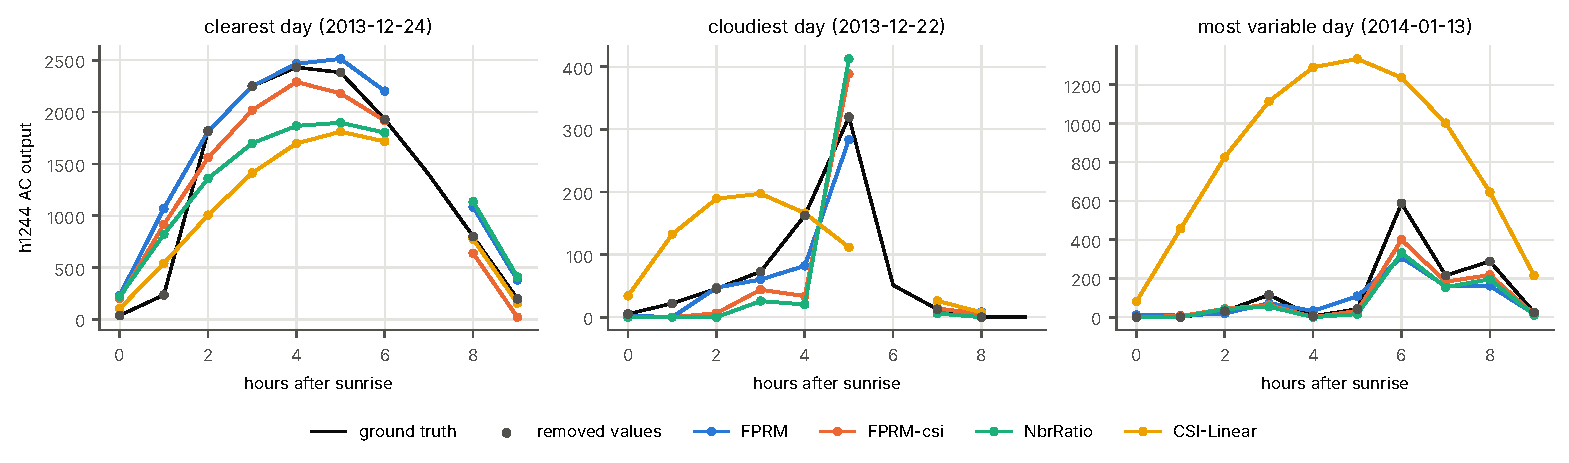
\includegraphics[width=\linewidth]{example_nola_1h_S6_r09.pdf}
  \caption{S6 복원 예(New Orleans 주택 1244, $r=0.9$, seed 0). 테스트일 중 가장 맑은 날, 가장 흐린 날, 변동이 가장 큰 날이다. 검정: 정답, 점: 제거된 값, 색 선: 제거된 시점의 복원값.}
  \label{fig:example}
\end{figure}

\subsection{실패 사례}\label{sec:failure}

\paragraph{고출력 구간 결측(S5 상위).}
주간 값의 상위 20\pct{}를 지운 경우는 포화·클리핑 손실의 단순 모형이다.
\begin{itemize}
  \item FPRM의 RMSE는 12.0--23.3\pct{}cap이다. 선형 이웃 기법(NbrOLS, NbrRatio)은 5.9--8.8\pct{}cap이다.
  \item 학습 데이터에 고출력 상태가 없으므로, GPR은 RF·$k$NN·SVR과 마찬가지로 학습 범위 밖을 외삽하지 못하고 평균 쪽으로 수축한다.
  \item 비례(선형) 모형은 자연스럽게 외삽된다.
  \item clear-sky 출력으로 정규화하면 고출력 상태가 덜 극단적이 되므로, 이 경우 FPRM-csi가 더 강건하다(평균 순위 5.8).
\end{itemize}

\paragraph{시간대 쏠림(S4, $P\ge4$).}
하루 24 step 중 $P$개마다 1개만 남기면 관측이 고정된 몇 시간대에만 남는다.
그 시간대 안에서의 교차검증은 큰 $E$와 $\tau$를 고르는데, 이렇게 고른 임베딩은 관측되지 않은 끌개 영역으로 일반화되지 않는다.
예컨대 Maui(1시간, $P=8$)에서 FPRM은 14.2\pct{}cap으로, FPRM-E1(8.7)과 NbrOLS(5.7)보다 나쁘다.
같은 이유로 Diurnal 베이스라인은 관측되지 않은 시간대에 대한 정보가 전혀 없어 에너지 오차가 100\pct{}가 된다.

\paragraph{동시 장애(S7).}
완전 관측 참조가 없으면 FPRM은 복원할 수 없다. 원 논문도 인정한 한계이며, 모든 FPRM 변형이 대체 방법과 같은 결과를 낸다.
여기서는 이웃 날짜의 같은 시각 평균(Diurnal)이 가장 좋다(평균 순위 3.9).

\paragraph{수치 발산.}
MICE는 S4에서 수치적으로 발산했다(RMSE가 $10^{45}$ 규모).
결과를 순위와 중앙값으로 요약한 이유다.

\subsection{Ablation과 참조 선택}\label{sec:ablation}

\Cref{tab:ablation}은 구성 요소를 하나씩 바꾼 결과다.
\begin{itemize}
  \item GPR을 SVR이나 MLP로 바꿔도 정확도는 거의 같다(8.73, 8.76 대 8.67\pct{}cap). 원 논문의 SVM$^*$/NN$^*$ 결과와도 부합한다. SVR은 약 45배 빠르다.
  \item 인과적(과거 방향) 임베딩도 정방향만큼 정확하므로, FPRM을 실시간으로 쓸 수 있다.
  \item clear-sky index 변환은 평균적으로 도움이 되지 않는다.
  \item 효과가 가장 큰 것은 참조 선택이다. S1/S2에서 지정 GHI 일사계를 참조로 고정하면 Maui의 RMSE가 5.5--7.6에서 16.3--17.7\pct{}cap으로 오른다. New Orleans와 St.\ Petersburg의 지정 이웃 참조는 0.3--0.7포인트 차이에 그친다.
\end{itemize}

S8 스윕(\cref{tab:refsweep})은 이를 일반화한다.
\begin{itemize}
  \item 참조 31개 \emph{모두}에서 임베딩이 FPRM-E1보다 4.8--29.6\pct{} 낫다.
  \item FPRM-ref는 New Orleans와 Maui에서는 모든 참조에 대해 NbrRatio를 이긴다.
  \item 네 사이트의 출력 프로파일이 거의 비례하는 St.\ Petersburg에서는 어느 참조로도 NbrRatio를 이기지 못한다.
  \item Maui에서 GHI 일사계는 단연 최악의 참조다(15.7--17.4\pct{}cap, 인버터 참조는 6.2--13.7).
\end{itemize}

\begin{table}[t]
  \centering\small
  \caption{FPRM ablation(S1 $r\in\{0.5,0.9\}$, S2 $L\in\{6,24\}$\,h, S6 $r\in\{0.5,0.9\}$; 데이터셋 4개, seed 3개). RMSE는 \%cap, 시간은 결측 시계열당 학습+예측 시간(CPU 1코어). $^\dagger$: 원 논문에 없음.}
  \label{tab:ablation}
  \input{\tabdir/ablation}
\end{table}

\begin{table}[t]
  \centering\small
  \caption{S8 참조 스윕(S6 마스크, $r=0.5$, seed 2개). 참조별 RMSE(\%cap)의 범위와 (평균), FPRM-E1 대비 FPRM-ref의 상대 이득 평균(최소, 최대), FPRM-ref가 NbrRatio를 이긴 참조 수.}
  \label{tab:refsweep}
  \resizebox{\linewidth}{!}{\input{\tabdir/refsweep}}
\end{table}

\section{논의}\label{sec:discussion}

\paragraph{일반 결측에서 표준 회귀기가 이기는 이유.}
이웃 태양광 시계열은 같은 구름장을 공유하며 상관이 0.97--0.99에 이른다.
따라서 여러 이웃의 순간값만으로 목표 상태가 거의 결정되고, 이웃 \emph{하나}의 지연 좌표가 더해 주는 정보는 이웃을 더 쓰는 것보다 작다.
둘을 결합한 FPRM-multi가 격차 대부분을 회복한다는 점은, 태양광에서 FPRM의 유용한 부분이 단일 참조 제약이 아니라 지연 임베딩임을 시사한다.

\paragraph{FPRM이 버리는 정보.}
FPRM은 입력이 완전해야 하므로, 값이 몇 개만 빠진 이웃도 쓸 수 없다.
실제 발전 단지에서 이웃이 한꺼번에 모두 결측되는 일은 드물다.
MICE가 부분 관측 시계열을 활용해 이긴 S6 $r=0.5$ 결과는 가장 유망한 확장 방향을 가리킨다.
결측 좌표를 허용하는 임베딩, 또는 복원된 이웃을 다시 참조로 넣는 반복 방식이다.

\paragraph{물리량 참조가 더 좋은 참조는 아니다.}
현장 일사계는 직관적으로 태양광 출력의 가장 ``물리적인'' 예측변수지만, 실제로는 최악의 참조였다.
설치면 방향, 음영, 시계 정합의 차이 때문에 일사계는 같은 지붕의 어떤 인버터보다도 어레이 상태를 덜 반영한다.
참조는 관측 구간 상관을 기준으로 데이터에 근거해 골라야 한다.

\paragraph{권장 파이프라인.}
결측 패턴에 따라 복원 방법을 분기한다.
\begin{itemize}
  \item 단지 전체 장애: Diurnal 또는 CSI 보간.
  \item 고출력·클리핑 손실 의심: NbrOLS 또는 NbrRatio.
  \item 완전 시계열이 적고 나머지 결측이 심함: FPRM. SVR을 쓰고, 상관이 가장 높은 참조를 고르며, 실시간이면 인과적 임베딩을 쓴다.
  \item 그 외: 모든 완전 이웃에 대한 RF/SVR 또는 FPRM-multi. 앙상블로 결합할 수도 있다.
\end{itemize}

\section{한계}\label{sec:limitations}
\begin{itemize}
  \item \textbf{데이터 접근.} NREL PVDAQ 데이터만 접근할 수 있었다. 다른 기후대, 대규모 발전소, 국내 발전 단지, 위성 일사량을 활용한 검증은 남아 있다.
  \item \textbf{원 코드.} 저자들의 MATLAB 코드 및 보충자료와 대조하지 못했고, Lorenz 수치는 원 논문과 다르다.
  \item \textbf{seed와 구간 길이.} seed 5개(ablation 3개)와 5--6개월 구간을 썼다. 1년 단위 시계열이라면 GPR의 학습점 상한(subset of data)이 더 큰 제약이 된다.
  \item \textbf{임베딩 선택.} 교차검증으로 고른 $(E,\tau)$가 seed에 따라 달라지므로($E=2$--8), 선택 과정이 분산의 원인이 된다.
  \item \textbf{미평가 확장.} lag-FPRM, S-map/MVCM, 딥러닝 대치(BRITS, SAITS)는 평가하지 않았다.
\end{itemize}

\section{결론}
동역학 기반 결측 복원은 태양광 데이터에도 부분적으로 통한다.
FPRM의 핵심인 지연 임베딩은 같은 회귀기의 성능을 일관되게 높이며, 결측이 심한 가운데 완전 시계열이 하나만 남은 상황에서는 FPRM을 최고의 방법으로 만든다.
그러나 일반적인 태양광 모니터링에서는 완전 관측 이웃이 여럿 있다.
이때 원 논문의 단일 참조 설계는 모든 이웃을 쓰는 표준 회귀기에 뒤지고, 고출력 결측, 시간대 쏠림 로깅, 동시 장애에서는 실패한다.
따라서 FPRM은 결측 패턴을 고려하는 복원 파이프라인 안에서, 가급적 다중 참조 형태의 특화 구성 요소로 쓰는 것이 바람직하다.

\section*{데이터 및 코드 가용성}
모든 데이터는 공개된 NREL PVDAQ 데이터셋~\cite{pvdaq}(OEDI, CC BY 4.0)이다.
코드, 전처리된 데이터셋, (재생성 가능한) 마스크, 원시 결과, 그리고 이 논문의 모든 표와 그림을 만드는 스크립트는 \url{https://github.com/jk-60hz/Wu-2026-missing-data}에서 받을 수 있다.

\section*{저자 기여 및 AI 활용 고지}
김종규는 연구를 기획하고, 연구 질문과 평가 설계를 정했으며, 결과와 원고를 검토했다.
Anthropic이 개발한 AI 시스템인 Claude Opus 5.5는 김종규의 지시에 따라 다음 작업을 수행했다.
\begin{itemize}
  \item FPRM과 벤치마크 구현
  \item 데이터 수집과 전처리
  \item 모든 실험 수행과 결과 분석
  \item 영문·국문 원고 초안 작성
\end{itemize}
이 논문의 모든 수치는 공개된 결과 파일에서 공개된 스크립트로 생성되었다.

\bibliographystyle{unsrtnat}
\bibliography{../refs}

\clearpage
\appendix
\section{추가 결과}

\begin{table}[h]
  \centering\small
  \caption{제거된 주간 구간의 총에너지 절대 오차 중앙값(정답 에너지 대비 \%). 굵은 글씨: 열별 최고.}
  \label{tab:energy}
  \input{\tabdir/energy}
\end{table}

\begin{table}[h]
  \centering\small
  \caption{데이터셋별 평균 순위(전체 시나리오). 굵은 글씨: 열별 최고.}
  \label{tab:rank_ds}
  \input{\tabdir/rank_by_dataset}
\end{table}

\begin{table}[p]
  \centering\scriptsize
  \caption{모든 시나리오·파라미터의 주간 RMSE(\%cap). 데이터셋, seed, 결측 시계열 평균. 굵은 글씨: 행별 최고, ``div.'': 수치 발산(S4의 MICE).}
  \label{tab:full}
  \resizebox{\linewidth}{!}{\input{\tabdir/full}}
\end{table}

\begin{figure}[p]
  \centering
  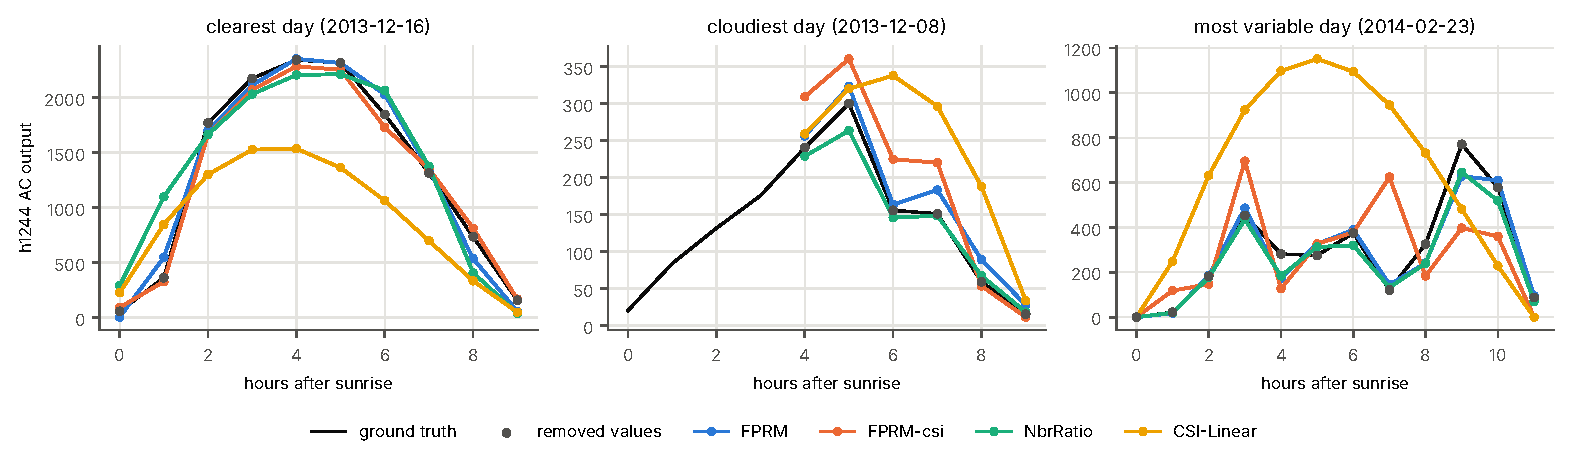
\includegraphics[width=\linewidth]{example_nola_1h_S2_24h.pdf}\\[-1pt]{\small (a) New Orleans, S2 $L=24$\,h}\\[4pt]
  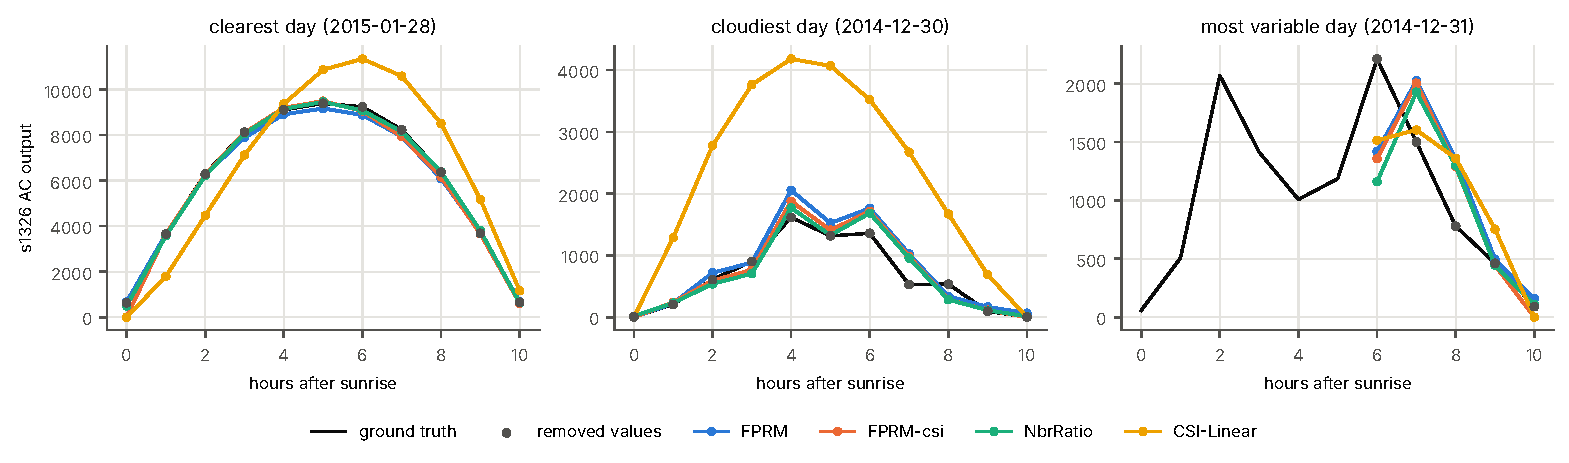
\includegraphics[width=\linewidth]{example_stpete_1h_S2_24h.pdf}\\[-1pt]{\small (b) St.\ Petersburg, S2 $L=24$\,h}\\[4pt]
  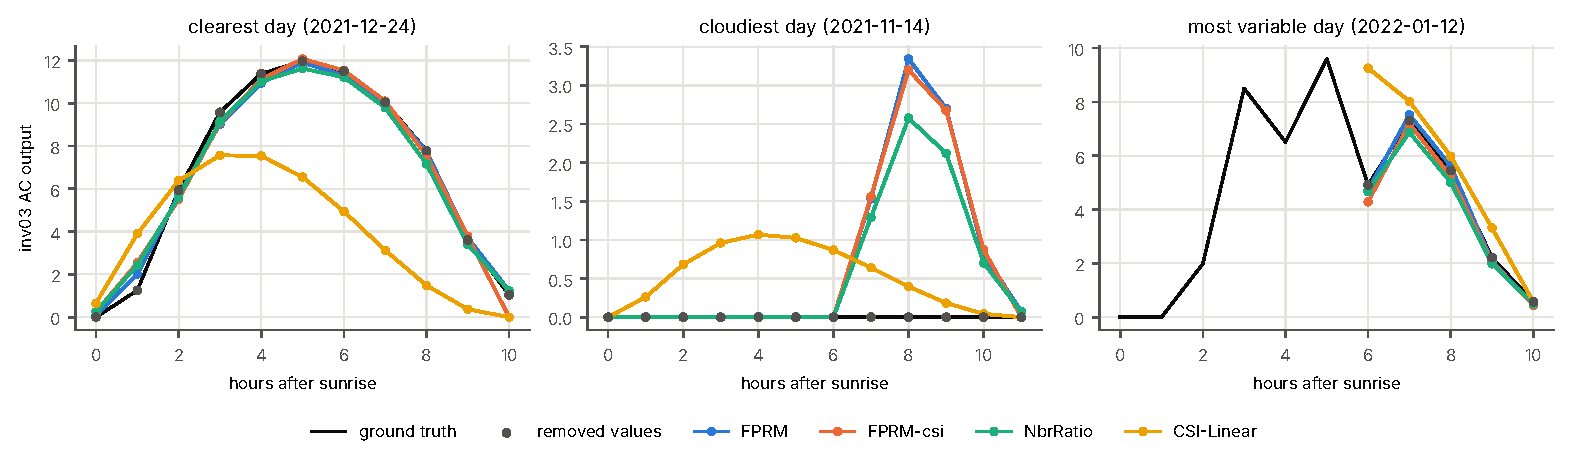
\includegraphics[width=\linewidth]{example_maui_1h_S2_24h.pdf}\\[-1pt]{\small (c) Maui 1\,h, S2 $L=24$\,h}\\[4pt]
  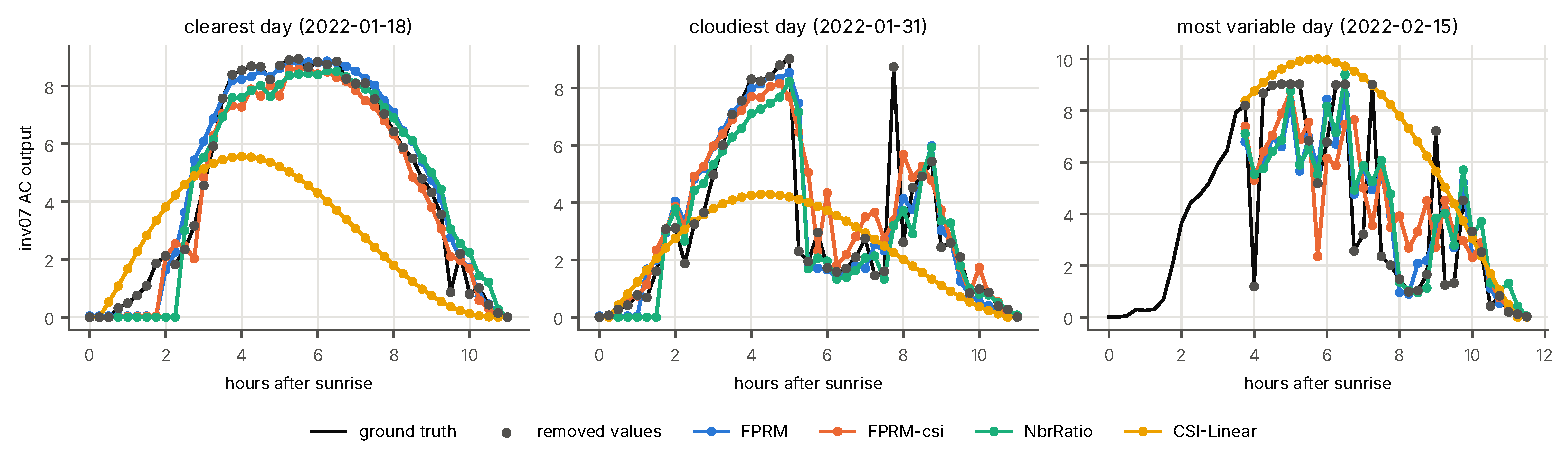
\includegraphics[width=\linewidth]{example_maui_15min_S2_24h.pdf}\\[-1pt]{\small (d) Maui 15\,min, S2 $L=24$\,h}
  \caption{24시간 공백의 복원 예(seed 0, 첫 번째 결측 시계열). 데이터셋마다 테스트일 중 가장 맑은 날, 가장 흐린 날, 변동이 가장 큰 날이다.}
  \label{fig:ex_s2}
\end{figure}

\begin{figure}[p]
  \centering
  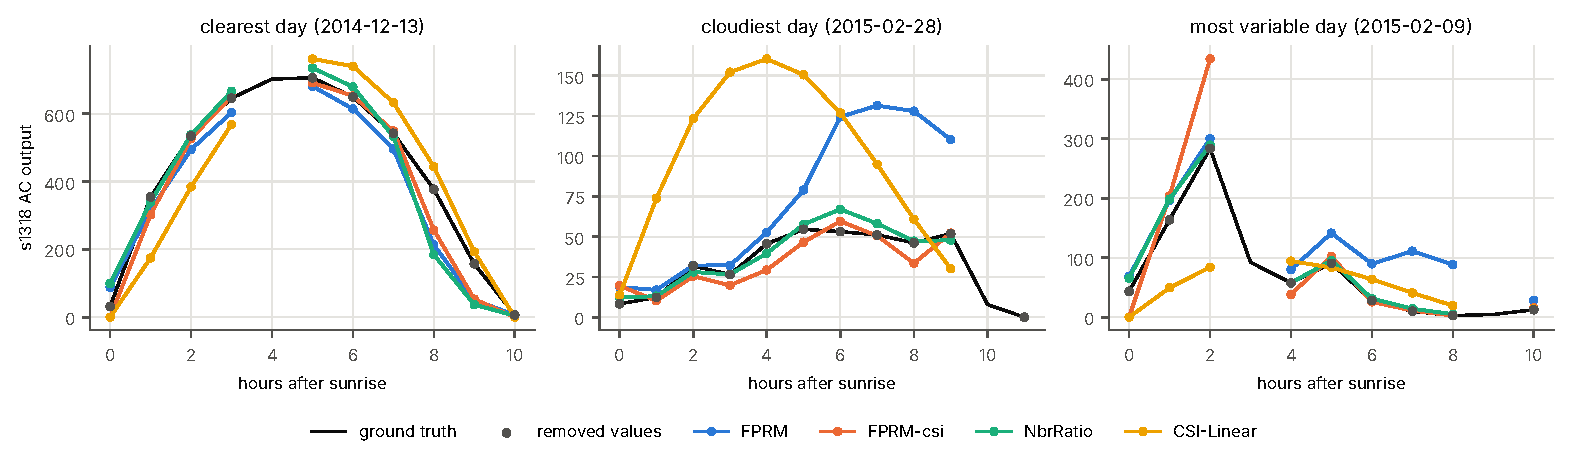
\includegraphics[width=\linewidth]{example_stpete_1h_S6_r09.pdf}\\[-1pt]{\small (a) St.\ Petersburg, S6 $r=0.9$}\\[4pt]
  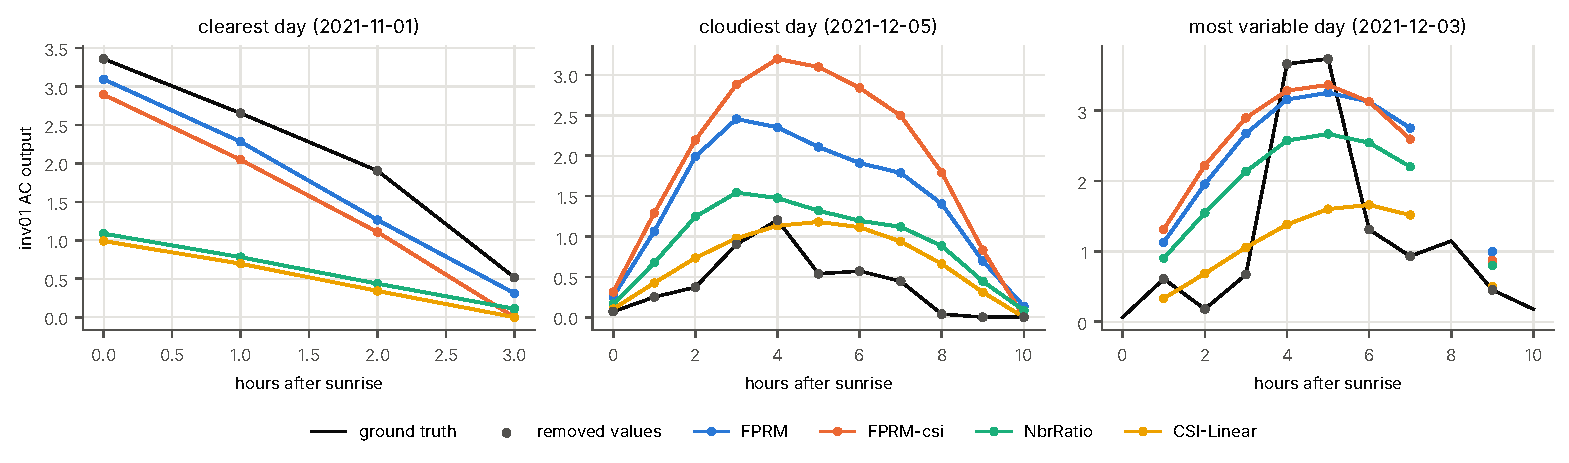
\includegraphics[width=\linewidth]{example_maui_1h_S6_r09.pdf}\\[-1pt]{\small (b) Maui 1\,h, S6 $r=0.9$ (참조: GHI)}\\[4pt]
  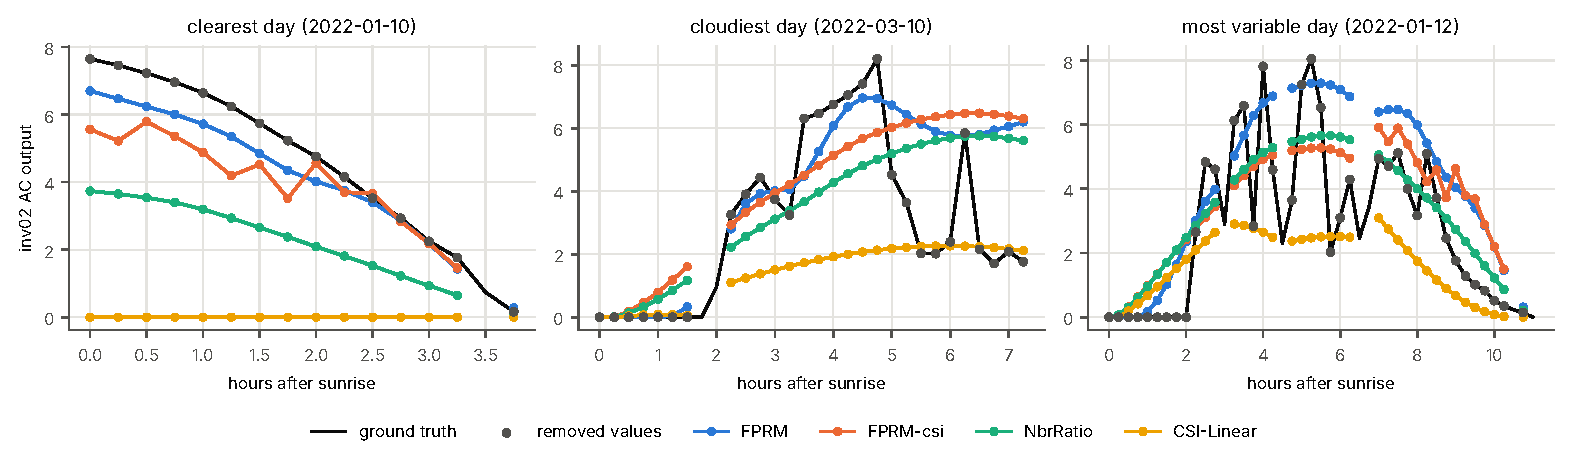
\includegraphics[width=\linewidth]{example_maui_15min_S6_r09.pdf}\\[-1pt]{\small (c) Maui 15\,min, S6 $r=0.9$ (참조: GHI)}
  \caption{$r=0.9$에서의 S6 복원 예(seed 0, 첫 번째 결측 시계열).}
  \label{fig:ex_s6}
\end{figure}

\section{재현 방법}
{\small\begin{verbatim}
python -m pytest -q tests
python scripts/reproduce_synthetic.py --reps 20 --workers 4
python scripts/make_testsets.py --seeds 5 \
    --datasets maui_15min,maui_1h,stpete_1h,nola_1h
python scripts/run_benchmark.py --config configs/main.yaml
python scripts/run_benchmark.py --config configs/ablation.yaml
python scripts/make_report.py --paper     # 논문 그림
python scripts/make_tables_tex.py         # 논문 표
\end{verbatim}}
CPU 4코어 기준으로 본 실험은 약 3시간, ablation은 약 1시간 걸린다.

\end{document}
